\documentclass[a4paper,10pt]{scrreprt}
%\documentclass{beamer}
\usepackage{graphicx} % Required for inserting images
\usepackage{amsmath}
\usepackage[siunitx,european]{circuitikz}
\usepackage[german]{babel}
% \usepackage[sc]{mathpazo}
% \linespread{1.05}   % Palladio needs more leading (space between lines)
% \usepackage{fourier}
% \usepackage{tgschola}
% \usepackage{times}
\usepackage[T1]{fontenc}
\usepackage{eurosym}
\usepackage{graphicx}
\usepackage{ulem}
\usepackage[pdfborder={0 0 0},colorlinks=true,linkcolor=blue]{hyperref}

% \usepackage{listings}
% Title Page
\begin{document}
  \title{Situationsbeschreibung der Firmengruppe TKmin}
\author{Thomas Maul}
\date{V 0.1 - im Aufbau\\ Stand: \today}%\\
\maketitle
\tableofcontents
\chapter{TKmin}
Die Firma TKmin  GmbH stellt hochwertige Tiefkühlprodukte für Endverbraucher und Großkunden her. Ihre Haupt Produktlinien sind Tiefkühlpizza und Eiscreme.

Im Hauptwerk gibt es drei Gebäude. Gebäude 1 ist die Verwaltung mit der Geschäftsleitung (GL). In Gebäude 2 ist die Produktion, in Gebäude 3 ist das Tiefkühllager (Rohwaren, Fertigprodukte)

\section{Netzwerk Verwaltungsgebäude}
Das Netzwerk ist historisch gewachsen und größtenteils auf Ethernet (CAT 5e) mit 1\,GB umgestellt worden. Der Plan in Bild \ref{fig:NetzwerkVerwaltung} zeigt das Netzwerk, das am allgemeinen Firmen-Netzwerk angeschlossen ist. Teile der Verwaltung (EG, Gang 2) sind noch ältere CAT 5 Kabel verlegt. Dort ist auch ein älterer 100 MB Switch. Dieser Teil ist am Netzwerk der Firma angeschlossen.

\subsection{Labor-Netzwerk}
In der Verwaltung, OG 1, Gang 3 ist ein altes Netzwerk mit 10MB, thin Ethernet. Das Netzwerk ist vom übrigen Netz der Firma abgekoppelt. Die PCs haben Win 3.11 und Win 95 - 98SE installiert. Das Netzwerk wird für spezielle Laborgeräte benötigt. Eine Umstellung der PCs ist nicht möglich.

\subsection{Server und Administrations-Bereich}
Im Verwaltungsgebäude (Keller) ist der SV und der GV der Verwaltung. Am GV ist auch das LAN der Administration und der Server angeschlossen. Der Server befindet sich in einem separaten Raum.

Im Keller gibt es einen Arbeitsraum für die Administration (mit Tageslicht) und den Serverraum.

\subsection{Weitere Stockwerke, Telefon}
Im allen Stockwerken des Gebäudes sind EV installiert. In Etage 1 und 2 gibt es 20 Büro mit je 2 PCs und zugehörigen Telefonen (alle VoIP).  Zusätzlich gibt es in allen Etagen je 5 WLAN-Access-Points.

\begin{figure}
 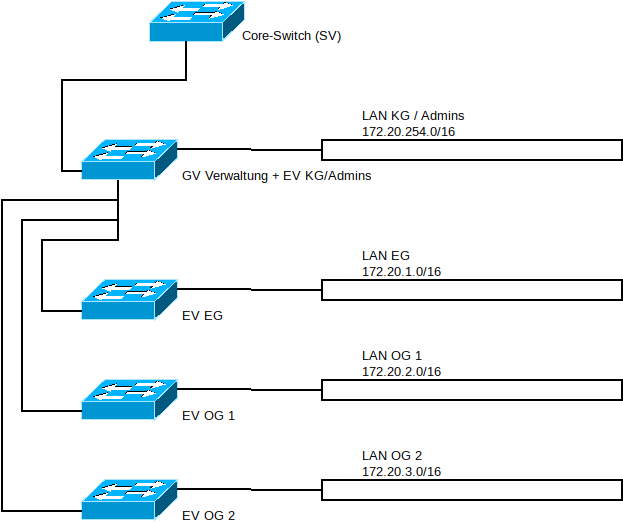
\includegraphics[width=.7\textwidth]{netzkplan_tkmin_verwaltung}
 % netzkplan_tkmin_verwaltung.ps: 683x436 px, 72dpi, 24.09x15.38 cm, bb=0 0 683 436
 \caption{Netzwerkplan Verwaltungsgebäude}
 \label{fig:NetzwerkVerwaltung}
\end{figure}

% \enlargethispage{\baselineskip}
\section{Backbone-Netzwerk}
Die Verbindung der Gebäude ist mit CAT 7 verlegt worden. Von Gebäude 1 zu Gebäude 2 ist die Leitung unterirdisch  verlegt, von Gebäude 1 zu Gebäude 3 oberirdisch (ca 5 m über dem Boden)

\section{Netzwerksegmente und Switches im LAN}
Das gesamte LAN der Firma ist im Bereich 172.120.0.0/16 installiert. Es gibt nur Switches. Ein Internet-Router verbindet den SV mit dem Internet (via ADSL 100k-Leitung).

Alle Switche im Firmen-LAN sind aktuelle Modelle namenhafter Hersteller. Der Switch in Verwaltung EG, Gang 2 ist ebenfalls von einem namenhaften Hersteller, er ist jedoch von 2000.

\section{Netzwerk Gebäude 2 und Gebäude 3}
Teile der Produktion sind aus technischen Gründen noch 10MB, Ethernet. Die Rechner der Maschinen können nicht getauscht werden, da sie Teil der Steuerung sind und Sicherheitsanforderungen unterliegen.

Die Übrigen Teile der Verkabelung sind CAT 7. Im LAN der Produktion (Gebäude 2) befindet sich ein GV (Netzwerkschrank nahe Eingang) und drei EV für die Teile der Produktion. An allen EV sind Maschinen und PCs der Linien-Leitung (Meister) angeschlossen.

\subsection{Gebäude 3}
In Gebäude 3 (Lager) befindet sich nahe der Eingangstür ein Netzwerkschrank mit dem GV. Da nur wenige PCs im Büro sind (aktuell 3 Stück) sind keine EV verbaut.

\section{Geschäftsleitung}
Die Geschäftsleitung besteht aus Dirk Schmidt. Er ist studierter Chemiker und hat große Erfahrung in der Lebensmitteltechnologie.

Leitung der IT-Abteilung ist Jasper Schmidt (Sohn vom Chef), er ist Fachinformatiker Systemintegration.

\section{Neues Personal und Unternehmenskultur}
Im Unternehmen erfolgt die Einarbeitung zur Zeit wie folgt:
Ein Mitglied der Geschäftsleitung oder der Personalabteilung begrüßt die neue Person in der Personalabteilung.

Die neue Person wird zum Arbeitsplatz begleitet und erhält dort als Ausdruck alle Zugangsdaten (persönliche und allgemeine für
Fernzugriff auf Server, ...). Unabhängig, welche Arbeiten die Person ausführen soll.

\begin{itemize}
 \item Die Person erhält einen Schlüssel zur Haustür.
 \item Sie wird informiert, welche Arbeiten sie durchführen soll und
 \item wo sich die Teeküche, Kantine und Toiletten befinden.
\end{itemize}

Das Unternehmen pflegt das Konzept der offenen Tür. Die Türen werden nur bei vertraulichen Gesprächen geschlossen.

\chapter{MiniPreis}
Die Firma TKmin GmbH hat – zur Stärkung des Absatzes – eine kleinere Kette von Supermärkten (Supermarkt MiniPreis GmbH) gekauft. MiniPreis  wird als eigenständige Firma weitergeführt.

Nach einer ersten Besichtigung wurde festgestellt, dass die IT-Infrastruktur vom MiniPreis angepasst werden soll. Um die Geschäftsabläufe zu optimieren, soll in mehreren Stufen die IT (unter anderem) vereinheitlicht werden.
\section{Ausgangssituation MiniPreis}

Die Supermarktkette MiniPreis hat in der Zentrale und einigen Filialen (Beispiel siehe Bild \ref{fig:GrundrissSupermarkt}) jeweils ein LAN mit dem IP-Bereich 192.168.240.0/24. Das Unternehmen war bei der Vernetzung bis jetzt etwas zurückhaltend. Der Datenaustausch erfolgt zurzeit noch per Papier, seit einigen Wochen auch per Versand von USB-Sticks.

Für die Umstellung sind folgende Schritte geplant:
\begin{enumerate}
 \item Datenaustausch per Cloud – soll zügig erfolgen (Wunsch der Geschäftsleitung). \\DSGVO muss gewährleistet werden, Vorgabe vom Datenschutz.
 \item Vernetzung
 \begin{enumerate}
  \item via VPN.
  \item via eigener Leitung (falls notwendig)
 \end{enumerate}
\end{enumerate}

\section{Filialen}
Nach einer Besichtigung wurde festgestellt, das einige Filialen mit Layer-2 Switchen vernetzt sind (ältere CAT 5 Leitungen, UTP, F/UTP). Andere sind mit 10Base2 vernetzt.

In der Filiale sind in der Regel folgende Netzwerkgeräte:
\begin{itemize}
 \item 3 PCs (Filialleitung, Personal-PC),
 \item 3 Kassen (mit jeweils einem PC),
 \item 4 Drucker (3 Bon-Drucker, 1 Laser für Filialleitung),
 \item 5 Kühlgeräte an drei Positionen (Steuerung soll per Fernwartung erreichbar sein),
 \item 1 Server (mit USV\footnote{Teilweise sind die USV der Server Netzwerkfähig}),
 \item 1 Layer-2 Switch (24 Port)
\end{itemize}

\section{Regionallager und Verwaltung}
An einem Standort befindet sich die Filiale in einem Gebäude. Im Nachbargebäude ist ein Regionallager der Supermarktkette. Oberhalb der Filiale soll in zwei Geschossen die Verwaltung von MiniPreis einziehen.
Die drei Netzwerke (Filiale, Regionallager, Verwaltung) sollen gekoppelt werden. Dabei sollen die Netze aber nicht zu einem großen Netzwerk verschmolzen werden.

\begin{figure}
 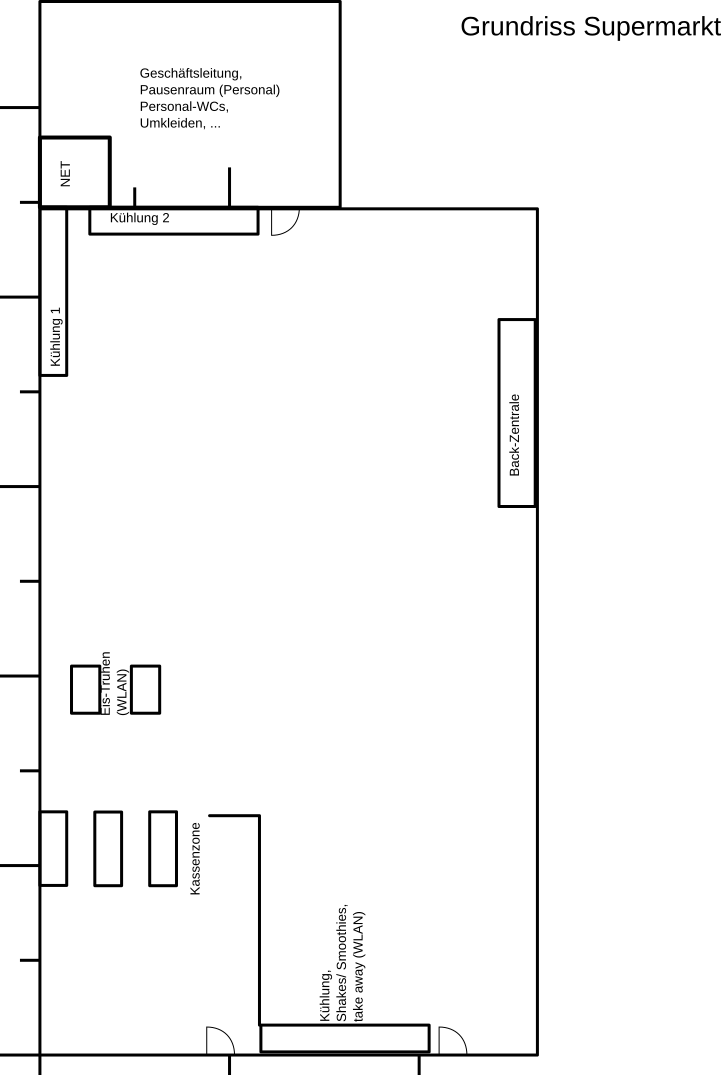
\includegraphics[width=.9\textwidth]{grundriss_supermarkt_v1_2.png}
 % grundriss_supermarkt_v1_2.png: 1075x618 px, 96dpi, 28.45x16.35 cm, bb=0 0 806 464
 \caption{Grundriß eines Supermarkts (Beispiel)}
 \label{fig:GrundrissSupermarkt}
\end{figure}

\section{Neustrukturierung der IT}
In den Filialen der MiniPreis und der zentrale sollen mittelfristig nur noch Thinclients oder terminalartige Geräte verwendet werden. Die Server sollen zentral aufgestellt und gewartet werden.

\chapter{Rechenzentrum}
Die IT-Abteilung der Firma TKmin nimmt unter dem Namen TopIT Aufträge von externen Auftraggebern an. Dies können Behörden, Firmen und Privatpersonen sein.

Die Geschäftsleitung von TopIT hat sich entschlossen für die Server der Firmen TKmin und MiniPreis ein eigenes kleineres Rechenzentrum zu errichten. Das Rechenzentrum ist in einem ehemaligen Wohn- und Bürogebäude am Stadtrand. Das Gebäude ist viergeschossig. Im Keller waren früher Aktenlager, im Erdgeschoss, ersten und zweiten OG waren Büros. Im dritten OG ist eine Wohnung, Sie wird renoviert und soll in ca. 3 Monaten bezogen werden (an extern vermietet).

Für TKmin gibt es einen physikalischen Server mit 6 VM (Datenbank, Dateiserver, AD mit Win Server, VoIP (Linux mit Asterisk), zwei Test-Server (für Azubis, einer mit Linux, einer mit Win-Server)). Der physikalische Server hat 3 HE. Für den Kunden MiniPreis sollen zwei weitere physikalische Server angeschafft werden.

\section{Lage des Gebäudes}
Das Gebäude liegt benachbart zu den Gebäuden von Minipreis (benachbartes Grundstück, es ist kein öffentlicher Weg zwischen den Grundstücken). Die Energieversorgung ist in Ordnung, wird von den Stadtwerken (Energieversorger, Versorger für Wasser, Fernwärme und Gas) geliefert (keine redundante Versorgung möglich).

Das Gebäude befindet sich an einem Hang (ca. 10 \% Gefälle). Der Hang ist oberhalb und unterhalb ca 30 m lang. Im Keller ist eine automatische Hebeanlage für Abwasser und Regenwasser. Der Boden ist felsig. Unterhalb des Gebäudes wurde eine Zisterne für Regenwasser angelegt.

Im Rechenzentrum sind in 2 Räumen im Untergeschoss (Keller) Server von Kunden aufgestellt. In weiteren 2 Räumen im EG und 5 Räumen im ersten OG sind ebenfalls Räume für Server vorgesehen. Im zweiten OG sind Büros eingerichtet. Sie verfügen über CAT 7 Verkabelung. Die Netzwerkgeräte (Switch, Router) sind ca. 3 Jahre alt und alle von einem namhaften Hersteller. Sie sind vollfunktionsfähig, GiB tauglich, alle Switch verfügen über min. ein SFP-Slot. 5 der 10 Geräte sind auf 24 (von 24) Ports 10 GiB tauglich. Sie haben 2 SFP-Slots. Der Router ist 10 GiB tauglich. Der Hausanschlussraum befindet sich im Keller. Dort terminiert auch die LWL des Internetproviders.

\section{Stromversorgung und Klimatisierung}
Die Stromversorgung erfolgt über eine Leitung, die oberirdisch angeschlossen ist (ca. 3,5 m über einem Feldweg). Neben der Leitung befindet sich auch die Glasfaserleitung für den Telefon- und Datenanschluss. Im Boden um das Gebäude herum befinden sich einige große Findlinge (je ca. 100 t - 200 t).

Die Server werden provisorisch über mobile Groß-Klimageräte gekühlt. Es ist geplant die Abwärme in das Netz der Fernwärme einzuspeisen, die benötigten Maschinen (Groß-Wärmepumpe) haben Lieferschwierigkeiten (ca. 3 Monate - Angabe vom Hersteller. Interne Voraussage (inoffiziell): voraussichtlich 6 Monate Lieferfrist. Es existiert eine alte Klimaanlage, die defekt aber reparaturfähig ist. Sie soll durch die Wärmepumpe ersetzt werden.

\section{Zugang zum Gebäude}
Der Zugangsschutz (zum Gebäude und Serverraum) wurde lange diskutiert. Es gibt zurzeit einen Schließzylinder mit Sicherungskarte (gegen unerwünschte Kopien). Alle Mitarbeitende haben einen Schlüssel erhalten. Die Schlüssel sind mit eingeprägten Zahlen fortlaufend nummeriert. Die Zuordnung der Schlüssel ist dokumentiert.

Für Notfälle befindet sich ein Ersatzschlüssel am hinteren Eingang des Bürogebäudes, außen im Treppenabgang zum Keller, in dem auch die Server stehen (unter dem Gitter des Lichtschachts 2, das Gitter klemmt, kann aber nicht verriegelt werden).

Die Straße ist auf der vorderen Seite des Gebäudes, der Feldweg von vorne gesehen rechts. Hinter dem Gebäude ist ein Grünstreifen mit dichter Wegetation (Bäume und Sträucher). Der Serverraum hat die gleiche Schließung, wie die Haustür.

Die Serverräume wurden früher als Wohnraum genutzt. Sie verfügen über eine Zentralheizung und Fenster. Da sie älterer Bauart (Baujahr ca. 1980) sind, klemmen sie teilweise. Die Fenster sind nicht mit Gittern oder Ähnlichem ausgestattet. Sie haben Rollzapfen als Verriegelung.

Zurzeit werden für die Büro-PCs der Firma TopIT Backups im Wochenrhythmus für die Büro-PCs erstellt. Die Erstellung erfolgt zentral auf ein NAS. Monatlich wird ein Vollbackup erstellt, wöchentlich ein differenzielles Backup.

\section{Entsorgungskonzept}
Alte Geräte und ausgemusterte Datenträger sollen in einem Raum gelagert werde und dann entsorgt werden. Zurzeit ist der Raum noch als Lager für Baumaterialien in Verwendung. Die ausgemusterten Geräte und Datenträger lagern zurzeit hinter dem Haus in einer Gitterbox. Die Gitterbox wurde mit einem Brett (formatfüllend) und einer Kette verschlossen. Sie werden ca. einmal pro Monat von einem Entsorgungsunternehmen abgeholt. Die Geräte werden nach Vorgaben des Elektroschrotts entsorgt. Die Entsorgung Elektroschrott wird dokumentiert und von einem zertifizierten Dienstleister übernommen.

Andere Abfälle werden sortiert nach Altpapier, Wertstoff ("grüner Punkt" und vergleichbar) und gemischte Wertstoffe (Hausmüllähnlicher Gewerbeabfall) über Container entsorgt. Die Container stehen im Hof. Der Hof ist offen, damit die Abfuhrfahrzeuge ungehindert die Abfallcontainer leeren können. Die Container werden in der Regel wöchentlich geleert.

\section{Videoüberwachung und Datenschutz}
Aus Datenschutzgründen sollten weder Hof noch Zufahrt videoüberwacht sein. Nach längeren Gesprächen mit MiniPreis wird das gesamte Gelände per Video überwacht. Die Aufzeichnungen werden auf einem NAS im OG (verschlossener Raum) gespeichert und automatisch nach drei Tagen gelöscht. Der Zugriff auf das NAS erfolgt nach dem 4 Augen-Prinzip.

Es gibt eine Datenschutzbeauftragte und einen Stellvertreter. Eine von beiden Personen muss sich mit einem persönlichen Hardware-Schlüssel und Passwort authentifizieren, um den Zugriff auf die Videoaufzeichnung zu ermöglichen. Falls beide Personen nicht erreicht werden können, kann die Löschung der Aufzeichnung für maximal 4 Wochen unterbrochen werden. Der Vorgang und alle Zugriffe auf das NAS werden extern in einem Rechenzentrum protokolliert. Die Authentifizierung erfolgt über einen Kerberos-Server. Der Hauptserver befindet sich im LAN des Rechenzentrums, der Backup-Server im externen Rechenzentrum.

Das externe Rechenzentrum ist ein gesicherter Raum in einem großen Rechenzentrum in Frankfurt. Der Backup-Server wird automatisch aktualisiert und ist als cold standby eingerichtet. Er übernimmt nach Aktivierung die Authentifizierung der Dienste. Der Zugriff ist über ein spezielles VPN per zwei-Faktor-Authentifizierung möglich. Die Authentifizierung erfolgt nicht über die Kerberos-Server.

\section{Netzwerk-Struktur}
Alle Switches sind VLAN fähig und min auf Layer 2 konfigurierbar. Es wurden noch keine VLANs eingerichtet. Switches, die 10 GiB tauglich sind haben 2 SFP-Slots und sind Layer 3 Switches. Sie verfügen über keine expliziten Routing-Funktionen.

In jedem Server-Rack befindet sich ein 10 GiB-tauglicher Switch. Alles Switches sind an einen zentralen Router angeschlossen. Im Büro-Bereich (2. OG) gibt es einen Switch, an den alle Büro-PCs  angeschlossen sind. Das Netzwerk ist über eine Firewall (FW, dezidiertes Gerät) nach außen abgesichert. Die FW wird automatisch aktualisiert.

Das Management der Switches, des Routers und der Firewall erfolgt über das Netzwerk 10.200.254/24. Dieses Netzwerk wird nicht geroutet. Die Admin-PCs in den Büros sind in diesem LAN eingetragen (zweite IP). Es gibt die Möglichkeit per Admin-VPN von außen auf das Netzwerk zuzugreifen. Zwei Laptops sind vor eingerichtet und bei den Personen, die Bereitschaftsdienst haben. Weitere Personen der Administration können sich mit Firmengeräten und zwei-Faktor Authentifizierung ebenfalls in das Netz-Management-LAN schalten.
\clearpage
Die Übrigen LANs sind wie folgt strukturiert:
\begin{itemize}
 \item 10.Etage.Raum+Rack.Gerät.
 \item Zweites Tupel: 99 = Keller, 100 = EG, 101 1. OG, 102 2. OG, 010 = 3. OG
 \item Im dritten Tupel ist die Raumnummer die erste und zweite Stelle. Es gibt maximal 9 Räume pro Etage. Die dritte Stelle ist die Rack-Nr. Wenn in einem Raum mehr als 9 Racks vorhanden sind, wird die Raumnummer mit 100 addiert, bei mehr als 19 Racks mit 200.
 \item Bei Büro-Geräten steht für das Rack immer die Nummer 1.
 \item Im 3. OG gibt es im dritten Tupel nur 001.
 \item Zukünftig sollen die IP-Adressen als Dualstack angelegt werden, alle Server sollen zeitnah auf Dualstack umgestellt werden. Vom ISP wurde ein Adress-Block 2001:8db:1234/48 zur Verfügung gestellt. Die Struktur mit Geschoss, Raum, Rack und Gerät soll in den IPv6-Adressen ebenfalls abgebildet werden.
\end{itemize}

Beispiel:
\\ Erdgeschoss, Raum 5, Rack 12, Server 15:
10.101.152.15 (eigentlich 052 + 100 für 10er-Stelle)

% \chapter{Rechenzentrum von TKmin}
% Die IT-Abteilung der Firma TKmin hat die Idee die Server der eigenen Firma und die von MiniPreis in einem eigenen, kleinen Rechenzentrum zu bündeln. Zusätzlich sollen Dienstleistungen für andere Kunden aus Industrie, Handel und Handwerk angeboten werden. Als Gebäude soll ein ehemaliges Büro- und Wohngebäude genutzt werden, das die Firma günstig erwerben konnte. Das Gebäude hat zwei Etagen (EG und OG) und ein Kellergeschoss.
%
% Im Gespräch sind folgende Optionen anzubieten:
% \begin{itemize}
%  \item Infrastructure as a Service
%  \item Platform as a Service
%  \item Software as a Service
% \end{itemize}
%
% Es ist geplant Server zu betreiben und die IT zentral zu verwalten und -- soweit möglich -- als private Cloud zu betreiben.
%
% Die Geschäftsleitung von TKmin hat sich entschlossen das vorgeschlagene kleinere Rechenzentrum zu errichten. Das Rechenzentrum ist in einer
% ehemaligen Bürogebäude am Stadtrand, auf dem benachbarten Grundstück zu den Gebäuden von Minipreis.
%
% \section{Lage des Gebäudes und Energieversorgung}
% Die Energieversorgung ist in Ordnung, wurde von den Stadtwerken (Energieversorger, Versorger für Wasser, Fernwärme und Gas) zugesichert.
%
% Das Gebäude befindet sich in einer Talsenke (ca 1m unter üblichen Gelände). Im Keller ist eine automatische Hebeanlage für Abwasser und
% Regenwasser.
%
% Die Stromversorgung erfolgt über eine Leitung, die oberirdisch angeschlossen ist (ca. 3,5 m über einem Feldweg). Neben der Leitung befindet sich auch die Glasfaserleitung für den Telefon- und Datenanschluss.
%
% Die Kühlung wird provisorisch über mobile Klimageräte gemacht, es ist geplant die Abwärme in das Netz der Fernwärme einzuspeisen, die
% benötigten Maschinen haben Lieferschwierigkeiten.
%
% \section{Zugang zum Gebäude}
% Der Zugangsschutz (zum Gebäude und Serverraum) wurde lange diskutiert. Es gibt einen Schließzylinder mit Sicherungskarte (gegen unerwünschte Kopien). Alle Mitarbeitende haben einen Schlüssel. Für Notfälle befindet sich ein Ersatzschlüssel am hinteren Eingang des Bürogebäudes, außen im Treppenabgang zum Keller, in dem auch die Server stehen. Die Straße ist auf der vorderen Seite des Gebäudes, der Feldweg von vorne gesehen rechts. Hinter dem Gebäude ist ein Grünstreifen mit dichter Wegetation (Bäume und Sträucher). Der Serverraum hat die gleiche Schließung, wie die Haustür. Aus Datenschutzgründen werden weder Hof noch Zufahrt videoüberwacht.
%
% \section{Serverräume}
% Im Rechenzentrum sind in 5 Räumen im Untergeschoss (Keller) Server von Kunden aufgestellt. Die Serverräume wurden früher als Wohnraum genutzt. Sie verfügen über eine Zentralheizung und Fenster. Da sie älterer Bauart (Baujahr ca 1980) sind, klemmen sie teilweise. Die Fenster sind nicht mit Gittern oder Ähnlichem ausgestattet. Sie haben Rollzapfen als Verriegelung.
%
% \section{Entsorgungskonzept}
% Alte Geräte und ausgemusterte Datenträger sollen in einem Raum gelagert werde und dann entsorgt werden. Zur Zeit ist der Raum noch als Lager für Baumaterialien in Verwendung. Die ausgemusterten Geräte und Datenträger lagern zur zeit hinter dem Haus in einer offenen Gitterbox. Sie werden ca. einmal pro Monat von einem Entsorgungsunternehmen abgeholt. Die Geräte werden nach Vorgaben des Elektroschrotts entsorgt. Die Entsorgung Elektroschrott wird dokumentiert und von einem Zertifizierten Dienstleister übernommen. Andere Abfälle werden sortiert nach Altpapier, Wertstoff (“grüner Punkt” und vergleichbar) und Abfall zur Behandlung (Hausmüllähnlicher Gewerbeabfall) über Container entsorgt. Die Container stehen im Hof. Der Hof ist offen, damit die Abfuhrfahrzeuge ungehindert die Abfallcontainer leeren können. Die Container werden in der Regel wöchentlich geleert.


\end{document}
